\documentclass{article}

\usepackage{parskip}
\usepackage{amsmath}
\usepackage{amssymb}
\usepackage{xfrac}
\usepackage{gensymb}
\usepackage{tikz}
\usepackage{esvect}

\renewcommand{\contentsname}{Chapter 1 - Vectors \& Scalars}

\begin{document}

\newpage
    \tableofcontents
\newpage

\section{Introduction to Vectors \& Scalars}

\subsection{Vectors \& Scalars}

\textbf{Scalar} = Magnitude \\
\textbf{Vector} = Magnitude + Direction

Vectors are represented by arrows – tail and tip

\begin{tikzpicture}
    \draw[->](0,0) -- (3,0);
\end{tikzpicture}

Triangle addition:
$$ \hat{A} = 20 \text{ @ } 40 \degree\ \text{above} +\hat{x} $$

$ \hat{x} \rightarrow $ Unit vector gives direction with Magnitude 1 ''the x direction"

Vector B is 45 @ 60 \degree\ Right of $ +\hat{y} $

\subsection{Algebra as an alternative to Euclidean Geometry}

In order to add vectors, first break vectors into \underline{components}

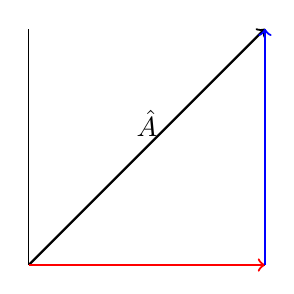
\begin{tikzpicture}
    \draw (0,0) -- (3,0)
          (0,0) -- (0,3);
    \draw[->, thick] (0,0) -- (3,3) node [midway, above] {$ \hat{A} $};
    \draw[->, thick, red] (0,0) -- (3,0);
    \draw[->, thick, blue] (3,0) -- (3,3);
\end{tikzpicture}

\underline{Any vector is the sum of its components}

\begin{equation}
    \boxed{\hat{A} = A_{x} \hat{x} + A_{y} \hat{y} + A_{z} \hat{z}} \\
\end{equation}
$$ \hat{A} = A \cos(\theta) \hat{x} + A \sin(\theta) \hat{y} \left( + 0 \hat{z} \right) $$

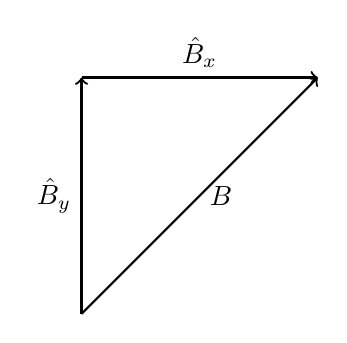
\begin{tikzpicture}
    \draw[->, thick] (0,0) -- (0,3) node [midway, left] {$ \hat{B}_{y} $};
    \draw[->, thick, rotate=45] (0,0) -- (4.242,0) node [midway, right] {$ \vv{B} $};
    \draw[->, thick] (0,3) -- (3,3) node [midway, above] {$ \hat{B}_{x} $};
\end{tikzpicture}

Write $ \vv{B} $ in component form:
$$ \vv{B} = B \sin(\phi) \hat{x} + B \cos(\phi) \hat{y} $$
$$ = (45) \sin(60\degree) \hat{x} + (45) \cos(60\degree) \hat{y} $$
\begin{equation*}
    \boxed{\vv{B} = 39 \hat{x} + 23 \hat{y}}
\end{equation*}

To add two vectors, add each direction separately:
$$ 15 \hat{x} + 13 \hat{y} $$
$$ 39 \hat{x} + 23 \hat{y} $$
$$ \vv{A} + \vv{B} = 54 \hat{x} + 36 \hat{y} $$

To substract two vectors, subtract each direction seperately:
$$ 15 \hat{x} + 13 \hat{y} $$
$$ 39 \hat{x} + 23 \hat{y} $$
$$ \vv{A} - \vv{B} = -24 \hat{x} - 10 \hat{y} $$

To compose (get magnitude and direction) of a vector, use:
$$ |\vv{A}| = \sqrt{ A_{x}^{2} + A_{y}^{2} + A_{z}^{2} } $$
$$ \theta_{\vv{A}} = \arctan \left( \frac{A_{i}}{A_{j}} \right) $$
$$ |\vv{A} + \vv{B}| = \sqrt{ (A + B)_{x}^{2} + (A+B)_{y}^{2} } $$
$$ = \sqrt{54^{2} + 36^{2}} = 65 $$
$$ \theta = \arctan \left( \frac{(A + B)_{y}}{(A + B)_{x}} \right) = \arctan \left( \frac{36}{54} \right) = 34\degree $$

\subsection{Scalar Multiplication}

$$ \gamma \vv{A} = \gamma A_{x}\hat{x} + \gamma A_{y}\hat{y} + \gamma A_{z}\hat{z} $$
$$ -\vv{A} = \left( -A_{x} \right)\hat{x} + \left( -A_{y} \right)\hat{y} + \left( -A_{z} \right)\hat{z} $$

Given three vectors connected from head to tail, find the distance from the tail of $ \vv{A} $ to the head of $ \vv{C} $:

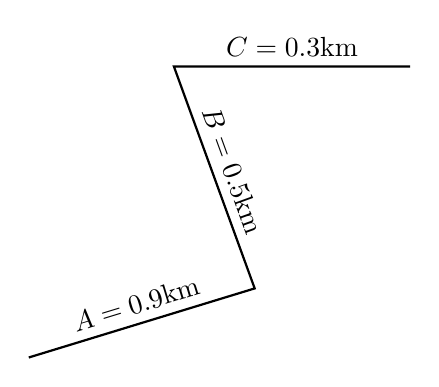
\begin{tikzpicture}
    \draw[thick] (0,0) -- (17:3cm) node [midway, above, sloped] {$ \vv{A} = 0.9 \text{km} $}
        -- ++(110:3cm) node [midway, above, sloped] {$ \vv{B} = 0.5 \text{km} $}
        -- ++(0:3cm) node [midway, above] {$ \vv{C} = 0.3 \text{km} $};
\end{tikzpicture}

\begin{align*}
    \vv{C} & = 0.3 \text{km} \hat{x} \\
    \vv{A} & = +A \cos(\theta) \hat{x} + A \sin(\theta) \hat{y} \\
           & = (0.9 \text{km}) \cos(17 \degree) \hat{x} + (0.9 \text{km}) \sin(17 \degree) \hat{y} \\
    \vv{A} & = 0.86 \text{km} \hat{x} + 0.26 \text{km} \hat{y} \\
    \vv{B} & = -B \sin(\phi) \hat{x} + B \cos(\phi) \hat{y} \\
    \vv{B} & = -0.17 \text{km} \hat{x} + 0.47 \text{km} \hat{y}
\end{align*}
\begin{align*}
    \vv{A} & = 0.86 \text{km} \hat{x} + 0.26 \text{km} \hat{y} \\
    \vv{B} & = -0.17 \text{km} \hat{x} + 0.47 \text{km} \hat{y} \\
    \vv{C} & = 0.3 \text{km} \hat{x} + 0 \hat{y}
\end{align*}
\begin{equation*}
    \boxed{\vv{A} + \vv{B} + \vv{C} = 0.99 \text{km} \hat{x} + 0.73 \text{km} \hat{y}}
\end{equation*}

\end{document}
